\chapter{The Helly property and EPG graphs}\label{cap:capiii}

\begin{flushright}
\begin{minipage}[t][0cm][b]{0.47\textwidth}
\emph{
%Talento é 1\% inspiração e 99\% transpiração. 
Genius is one percent inspiration, ninety nine percent perspiration.
}
\end{minipage}

\rule[0cm]{7cm}{0.03cm}%{largura}{espessura}

Thomas Edison
\end{flushright}

% Neste capítulo examinaremos as relações hierárquicas entre algumas classes EPG e EPG-Helly. Ademais, abordaremos representações $B_1$-EPG de alguns grafos que serão utilizados posteriormente. Primeiro, vamos observar como as classes $B_0$-EPG, $B_0$-EPG-Helly, $B_1$-EPG e $B_1$-EPG-Helly se relacionam, em seguida consideramos as representações $B_1$-EPG de $C_4$'s e do grafo octaedro. Por último, apresentaremos a prova de $NP$-completude do problema de reconhecimento de grafos $B_1$-EPG-Helly.

\begin{quotation}
In this chapter, we will examine the hierarchical relationships among some EPG and Helly-EPG classes. In addition, we will approach $ B_1$-EPG representations of some graphs that will be used later. First, let us focus our attention to understand how the classes $B_0$-EPG, $B_1$-EPG,  Helly-$B_1$ EPG, and  $L$-shaped paths are related, then we consider the $ B_1$-EPG representations of graphs $C_4 $ and the Octahedral graph. Next, we will present the proof of $NP$-completeness to Helly-$B_1$-EPG graph recognition problem. Finally, at the end of this chapter, the reader can find a section with a complete version of the paper published in the journal DMTCS that contains the set of proofs that have been omitted from the text.
\end{quotation}

\section{Introduction}
An EPG graph $G$ is a graph that admits a representation in which its vertices are represented by paths of a grid $Q$, such that two vertices of $G$ are adjacent if and only if the corresponding paths have at least one common edge.

The study of EPG graphs has motivation related to the problem of VLSI design that combines the notion of edge intersection graphs of paths in a  tree with a  VLSI  grid layout model, see~\cite{golumbic2009}. The number of bends in an integrated circuit may increase the layout area, and consequently, increase the cost of chip manufacturing.
This is one of the main applications that instigate research on the EPG representations of some graph families when there are constraints on the number of bends in the paths used in the representation.
Other applications and details on circuit layout problems can be found in~\cite{bandy1990, molitor1991}.

A graph is a $ B_k$-EPG graph if it admits a representation in which each path has at most $k$ bends. As an example, Figure~\ref{fig:trianguloepgRepresentacao}(a) shows a $C_3$, Figure~\ref{fig:trianguloepgRepresentacao}(b) shows an EPG representation where the paths have no bends and Figure~\ref{fig:trianguloepgRepresentacao}(c) shows a representation with at most one bend per path.   
Consequently, $C_3$ is a $B_0$-EPG graph. More generally, $B_0$-EPG graphs coincide with interval graphs.


\begin{figure}[h]
  \centering
  \begin{tabular}{ p{3cm} p{0.7cm} p{4cm} p{0.7cm} p{4cm} }
    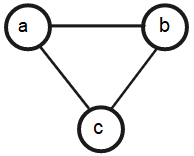
\includegraphics[width=2.3cm]{./img/trianguloabc} && 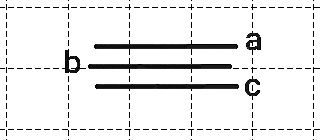
\includegraphics[width=3.9cm]{./img/b0epgTransparenciaGrade2} & &
    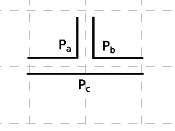
\includegraphics[width=3.5cm]{./img/b1EpgTransparenteGrade2}
    \\
    \footnotesize
    (a) The  graph $C_3$. && \footnotesize(b) $B_0$-EPG representation of $C_3$ (edge-clique).&& \footnotesize(c) $B_1$-EPG representation of $C_3$ (claw-clique).\\
  \end{tabular}

 \caption{The  graph $ C_3 $  and  representations without bends and with 1 bend.} \label{fig:trianguloepgRepresentacao}
\end{figure}


The \emph{bend number} of a graph $G$ is the smallest $k$ for which $G$ is a $B_k$-EPG graph. Analogously, the bend number of a class of graphs is the smallest $k$ for which all graphs in the class have a $B_k$-EPG representation. Interval graphs have bend number $0$, trees have bend number $1$, see~\cite{golumbic2009}, and outerplanar graphs have bend number $2$, see~\cite{daniel2014b}. The bend number for the class of planar graphs is still open, but according to \cite{daniel2014b}, it is either $3$ or $4$.

The class of EPG graphs has been studied in several papers, such as \cite{alcon2016, Asinowski2009, cohen2014, golumbic2009, heldt2014,  martin2017,golumbic2019edge}, among others. The investigations regarding EPG graphs frequently approach characterizations concerning the number of bends of the graph representations. Regarding the complexity of recognizing $B_k$-EPG graphs, only the complexity of recognizing a few of these sub-classes of EPG graphs have been determined: $B_0$-EPG graphs can be recognized in polynomial time, since it corresponds to the class of interval graphs, see ~\cite{booth1976}; in contrast, recognizing $B_1$-EPG and $B_2$-EPG graphs are NP-complete problems, see~\cite{heldt2014} and \cite{martin2017}, respectively. 
Also, note that the paths in a $B_1$-EPG representation have one of the following shapes: $\llcorner$, $\lrcorner$, $\ulcorner$ and $\urcorner$. \cite{cameron2016edge} showed that for each $S\subset \{\llcorner, \lrcorner, \ulcorner, \urcorner\}$, it is NP-complete to determine if a given graph $G$ has a $B_1$-EPG representation using only paths with shape in $S$.

A  collection $C$ of sets satisfies the Helly property when every sub-collection of $C$ that is pairwise intersecting has at least one common element. 
The study of the Helly property is useful in diverse areas of science. We can enumerate applications in semantics, code theory, computational biology, database, image processing, graph theory, optimization, and linear programming, see \cite{dourado2009}.

The Helly property can also be applied to the $B_k$-EPG representation problem, where each path is considered a set of edges. A graph $G$ has a  Helly-$B_k$-EPG representation if there is a $B_k$-EPG representation of $G$ where each path has at most $k$ bends, and this representation satisfies the Helly property. Figure~\ref{fig:envelopeRepresentacoes}(a) presents two $B_1$-EPG representations of a graph with five vertices.  Figure~\ref{fig:envelopeRepresentacoes}(b)   illustrates 3 pairwise intersecting paths ($P_{v_1}, P_{v_2}, P_{v_5}$), containing a common edge, so it is a Helly-$B_1$-EPG representation. In Figure~\ref{fig:envelopeRepresentacoes}(c), although the three paths are pairwise intersecting, there is no common edge in all three paths, and therefore they do not satisfy the Helly property.

The Helly property related to EPG representations of graphs has been studied in~\cite{golumbic2009} and~\cite{golumbic2013}. 

Let $\cal {F}$ be a family of subsets of some universal set $U$, and $h\geq 2$ be an integer.  Say that $\cal{F}$ is $h$-{\it intersecting} when every group of $h$ sets of $\cal {F}$ intersect. The {\it core} of $\cal {F}$, denoted by $core(\cal F)$, is the intersection of all sets of $\cal {F}$. The family $\cal{F}$ is $h$-{\it Helly} when every $h$-intersecting subfamily $\cal{F'}$ of $\cal{F}$ satisfies $core(\cal{F'}) \neq \emptyset$, see e.g. \cite{duchet1978propriete}. On the other hand, if for every subfamily $\cal{F'}$ of $\cal{F}$, there are $h$ subsets whose core equals the core of  $\cal {F'}$, then $\cal {F}$ is said to be {\it strong} $h$-{\it Helly}.
Note that the Helly property that we will consider in this paper is precisely the property of being 2-Helly. 

The  {\it Helly number} of the family $\cal{F}$ is the least integer $h$, such that $\cal{F}$ is $h$-Helly. Similarly, the {\it strong Helly number} of $\cal{F}$ is the least $h$, for which  $\cal{F}$ is strong $h$-Helly. It also follows that the strong Helly number of $\cal{F}$ is at least equal to its Helly number. In~\cite{golumbic2009} and~\cite{golumbic2013}, they have determined the strong Helly number of $B_1$-EPG graphs. 


\begin{figure}[h]
  \centering
  \begin{tabular}{ p{3.2cm} p{4.5cm} p{4.5cm} }
    \centering 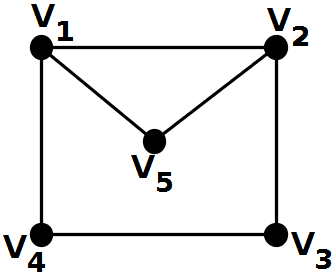
\includegraphics[width=3cm]{./img/envelope} & 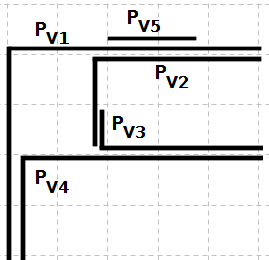
\includegraphics[width=4cm]{./img/envelopeHellyGradeTransparente} & 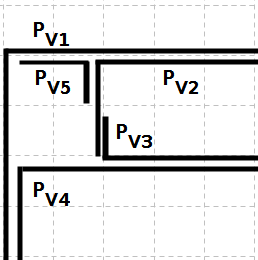
\includegraphics[width=4cm]{./img/envelopeNaoHellyGrade}
    \\
    \footnotesize \centering (a) A  graph with 5 vertices. & \footnotesize(b) A $B_1$-EPG representation that satisfies the Helly property. & \footnotesize (c) A $B_1$-EPG representation that does  not satisfy the Helly property.  \\

  \end{tabular}
\caption{A  graph with 5 vertices in (a) and some single bend representations: Helly in (b) and not Helly in (c).} \label{fig:envelopeRepresentacoes}
\end{figure}

%%%%%%%%%%%%%%%%%%%%%%%%%%%%%%%%%%%%%%%%%%%%%%%%%%%%%%%%%%%%%


Next, we describe some terminology and notation.

The term \emph{grid} is used to denote the Euclidean space of integer orthogonal coordinates. Each pair of integer coordinates corresponds to a \emph{point} (or vertex) of the grid. The \emph{size} of a grid is its number of points. The term \emph{edge of the grid} will be used to denote a pair of vertices that are at a distance one in the grid. Two edges $e_1$ and $e_2$ are \emph{consecutive edges} when they share exactly one point of the grid.
 A (simple) path in the grid is as a sequence of distinct edges $e_1, e_2, \leq, e_m$,  where consecutive edges are adjacent, i.e., contain a common vertex, whereas non-consecutive edges are not adjacent.  In this context, two paths only intersect if they have at least a common edge. The first and last edges of a path are called \emph{extremity edges}.
  
The \emph{direction of an edge} is vertical when the first coordinates of its vertices are equal, and is horizontal when the second coordinates are equal. A \emph {bend} in a path is a pair of consecutive edges $ e_1, e_2 $ of that path, such that the directions of $ e_1$ and $ e_2$ are different. When two edges $ e_1$ and $e_2 $ form a bend, they are called \emph { bend edges}. A \emph {segment} is a set of consecutive edges with no bends. %is a path with no bends.
Two paths are said to be \emph{edge-intersecting}, or simply  \emph{intersecting} if they share at least one edge. Throughout the paper, any time we say that two paths intersect, we mean that they edge-intersect. If every path in a representation of a graph $G$ has at most $k$ bends, we say that this graph $G$ has a \emph{$B_k$-EPG} representation. When $k = 1$ we say that this is a \emph{single bend} representation.

\medskip

In this chapter, we study the Helly-$B_k$-EPG graphs. First, we show that every graph admits an EPG representation that is Helly, and present a characterization of Helly-$B_1$-EPG representations. Besides, we relate Helly-$B_1$-EPG graphs with L-shaped graphs, a natural family of subclasses of $B_1$-EPG. Finally, we prove that recognizing Helly-$B_k$-EPG graphs is in NP, for every fixed $k$. Besides, we show that recognizing Helly-$B_1$-EPG graphs is NP-complete, and it remains NP-complete even when restricted to 2-apex and 3-degenerate graphs.

The rest of the chapter is organized as follows. In Section~\ref{sec:prelim}, we present some preliminary results, we show that every graph is a Helly-EPG graph, present a characterization of Helly-$B_1$-EPG representations, and relate Helly-$B_1$ EPG with L-shaped graphs. In Section~\ref{sec:NPpert}, we discuss the NP-membership of {\sc Helly-$B_k$ EPG Recognition}. In Section~\ref{sec:sectionDispositivoClausula}, we present the NP-completeness of recognizing Helly-$B_1$-EPG graphs. Finally, in the last section the reader can find the complete paper accepted to  journal Discrete Mathematics \& Theoretical Computer Science (DMTCS) that contains the set of proofs that have been omitted from the text.


\section{Preliminaries} \label{sec:prelim}

Before leaving for more laborious results to obtain, let us first notice a simple result. We can observe that when we do not restrict the number of bends of each path, we can show that any graph can be represented as an EPG graph.

This study starts with the following lemma.

\begin{lemma}[\citet{golumbic2009}] \label{lem:todoGrafoEpg}
 Every graph is an EPG graph.
 \end{lemma}
 
 Moreover, the same applies to EPG-Helly graphs. 
 
In an equivalent way, it is also possible to show that every graph has an EPG representation that satisfies the Helly property. An algorithm that performs this construction is presented in the Lemma~\ref{lem:todoGrafoEpgHelly}.

 \begin{lemma}\label{lem:todoGrafoEpgHelly}
 Every graph is a Helly-EPG graph.
 \end{lemma}

% \begin{proof}
% Let $G$ be a graph with $n$ vertices $v_1, v_2, \dots, v_n$ and $\mu$ maximal cliques $C_1, C_2, \dots , C_{\mu }$. We construct a Helly-EPG representation of $G$ using a $\mu +1\times \mu +1$ grid $Q$. 
% %The rows and columns correspond to each maximal cliques and are numbered $1, 2, \dots , \mu$. 
% Each maximal clique $C_i$ of $G$ is mapped to an edge of $Q$ as follow: 
% \begin{itemize}
%     \item if $i$ is even then the maximal clique $C_i$ is mapped to the edge in column $i$ between rows $i$ and $i+1$;
%     \item if $i$ is odd then the maximal clique $C_i$ is mapped to the edge in row $i$ between columns $i$ and $i+1$.
% \end{itemize}

% The following describes a descendant-stair-shaped construction for the paths.
  
% Let $v_l \in V(G)$ and $C_i$ be the first maximal clique containing $v_l$ according to the increasing order of their indices. If $i$ is even (resp. odd) the path $P_l$ starts in column $i$ (resp. in row $i$), in the point $(i,i)$. Then $P_l$ extends to at least the point $(i+1, i)$ (resp. $(i, i+1)$) proceeding to the until the row (resp. column) corresponding to next maximal clique of the sequence containing $v_l$, we say $C_{j}$.
% At this point, we bend $P_l$, which goes to the point $(j,j)$ and repeat the process previously described. 
% %
% Figure~\ref{fig:gradeDemonstracao} shows the Helly-EPG representation of the octahedral graph $O_3$, according to the construction previously described.

% By construction, each path travels only rows and columns corresponding with maximal cliques containing its respective vertex. And, every path crosses the edges of the grid to which your maximal cliques were mapped. Thus, the previously described construction results in an EPG representation of $G$, which is Helly since every set ${\mathcal P}$ of paths representing a maximal clique has at least one edge in its core.
% \end{proof}
 
%  \begin{figure}[htb]	
\center%6.3
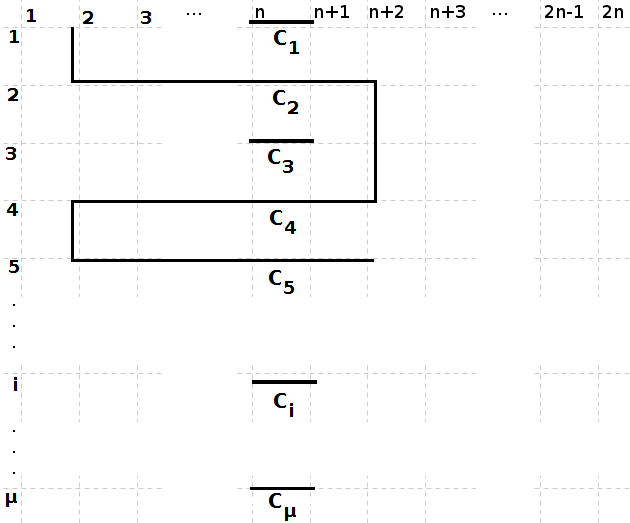
\includegraphics[width=8cm]{./img/grade3.png}
%clausulaGadgetGFCompletaSBPO
\caption{Representação do caminho $P_2$ correspondendo ao vértice $v_2$ contido nas cliques maximais $C_2, C_4$ e $C_5$}
\label{fig:gradeDemonstracao}
\end{figure}


 The provided construction in Lemma~\ref{lem:todoGrafoEpgHelly} can be modified to represent an monotonic row-ascendant EPG representation how in~\cite{golumbic2009} and~\cite{golumbic2013}. To do this, it is enough to change the orientation of the y-axis such that it grows from bottom to up.

%   The Helly property related to EPG representations of graphs has been studied in~\citet{golumbic2009,golumbic2013}.

\begin{definition}
The \emph{Helly-bend number} of a graph $G$, denoted by $b_H(G)$, is the smallest $k$ for which $G$ is a Helly-$B_k$-EPG graph. Also, the bend number of a graph class ${\mathcal C}$ is the smallest $k$ for which all graphs in ${\mathcal C}$ have a $B_k$-EPG representation.
\end{definition}
 
\begin{corollary}\label{cor:maxCliques}
For every graph $G$ containing $\mu$ maximal cliques, it holds that $b_H(G)\leq \mu -1$. 
\end{corollary}


The proof of Corollary~\ref{cor:maxCliques}  is immediate by the Lemma~\ref{lem:todoGrafoEpgHelly}.

Next, we examine the $B_1$-EPG representations of a few graphs that we employ in our constructions.

\medskip

Given an EPG representation of a graph $G$, for any grid edge $e$, the set of paths containing $e$ is a clique in $G$; such a clique is called an edge-clique. A claw in a grid consists of three grid edges meeting at a grid point. The set of paths that contain two of the three edges of a claw is a clique; such a clique is called a claw-clique, see~\cite{golumbic2009}. Fig.~\ref{fig:trianguloepgRepresentacao} illustrates an edge-clique and a claw-clique.

\begin{lemma}[\citet{golumbic2009}]\label{edge-claw-clique} 
Consider a $B_1$-EPG representation of a graph $G$. Every clique in $G$ corresponds to either an edge-clique or a claw-clique.
\end{lemma}

Next, we present a characterization of Helly-$B_1$-EPG representations.

\begin{lemma}\label{caracterization}
A $B_1$-EPG representation of a graph $G$ is Helly if and only if each clique of $G$ is represented by an edge-clique, i.e., it does not contain any claw-clique.
\end{lemma}

The Lemma~\ref{caracterization} is useful to prove that we can check if a given $B_1$-EPG representation is Helly. Just check each clique. 

Now, we consider EPG representations of $C_4$.

\begin{definition} \label{defi:tortasFrame}
Let $ Q $ be a grid and let $ (a_1, b),$ $(a_2, b),$ $(a_3, b),$ $(a_4, b)$ be a 4-star as depicted in Figure~\ref{fig:piesInGrid2}(a). Let $ \mathcal{P} = \{P_1, \dots , P_4\}$ be a collection of distinct paths each containing exactly two edges of the $4$-star.
\begin{itemize}
\item A \emph{true pie} is a representation where each $P_i$ of $ \mathcal{P} $ forms a bend in $b$.

\item A \emph {false pie} is a representation where two of the paths $P_i$ do not contain bends, while the remaining two do not share an edge. 
\end{itemize}
\end{definition}

Fig.~\ref{fig:piesInGrid2} illustrates true pie and false pie representations of a $C_4$.

\begin{figure}[htb]
  \centering
%segundo bloco de figuras
  \begin{tabular}{c c c c c }
    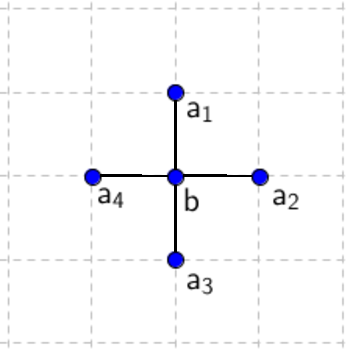
\includegraphics[width=3.5cm]{./img/disposicaoTortaGrid3}    
    & &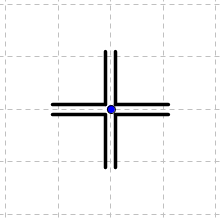
\includegraphics[width=3.5cm]{./img/truePieGrid} 
    & &
 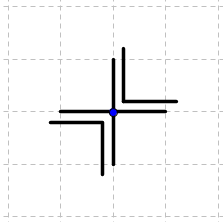
\includegraphics[width=3.5cm]{./img/falsePieGrid} \\%[\abovecaptionskip]
    {\footnotesize (a) 4-star in grid.}  & &  {\footnotesize (b) True pie.} & & {\footnotesize (c) False pie.} %\label{fig:frame}
  \end{tabular}
  \caption{$B_{1}$-EPG representation of the induced cycle of size 4 as pies with emphasis in center $b$.}\label{fig:piesInGrid2}
\end{figure} 


\begin{definition} \label{defi:tortasFrame2}
 Consider a rectangle of any size with 4 corners at points $ (x_1, y_1);$ $(x_2, y_1);$ $(x_2, y_2);$ $(x_1, y_2) $, positioned as in  Fig.~\ref{fig:frameInGrid}(a). 
 \begin{itemize}
 \item A \emph{frame} is a representation containing 4 paths $\mathcal{P} =  \{ P_1, \dots, P_4\} $, each having a bend in a different corner of a rectangle, and such that the  sub-paths $ P_1 \cap P_2, P_1 \cap P_3, P_2 \cap P_4, P_3 \cap P_4 $ share at least one edge. While $P_1 \cap P_4 $ and $ P_2 \cap P_3$ are empty sets.
 
 \item A square-frame is a frame where $P_1$, $P_2$, $P_3$ and $P_4$ have respectively point of bend $ (x_1, y_1),$ $(x_2, y_1),$ $(x_1, y_2)$ and $(x_2, y_2)$, and are of the shape $\llcorner$, $\lrcorner$, $\ulcorner$ and $\urcorner$.  (see Fig.\ref{fig:frameInGrid})
 \end{itemize}
\end{definition}

Fig.~\ref{fig:frameInGrid} illustrates some frame representations of a $C_4$.





\begin{figure}[htb]
  \centering
  \begin{tabular}{c c c c c }
    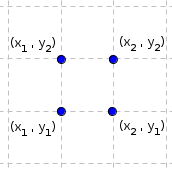
\includegraphics[width=3.5cm]{./img/dispositionFrameInGrid}    
    & &
   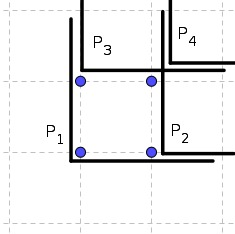
\includegraphics[width=3.5cm]{./img/frame2} 
     & &
   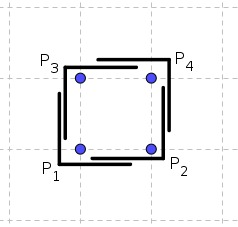
\includegraphics[width=3.5cm]{./img/square2} \\%[\abovecaptionskip]
   {\footnotesize (a) Coordinates of bends of a frame}  
   & & {\footnotesize (b) An example of a frame} 
   & & {\footnotesize (c) A square-frame} %\label{fig:frame}
  \end{tabular}
  \caption{$B_{1}$-EPG representation of the induced cycle of size 4 as frame}\label{fig:frameInGrid}
\end{figure} 


\begin{lemma}[\citet{golumbic2009}]\label{lem:representacaoC4}
Every  $C_4$ that is an induced subgraph of a graph $ G $ corresponds, in any representation, to a true pie, a false pie, or a frame.
\end{lemma}

The following is a claim of~\cite{heldt2014} which a reasoning can be found in~\cite{Asinowski2009}.

\begin{lemma}[\citet{daniel2014b} and \citet{Asinowski2009}]\label{fact:k24facts}
In every single bend representation of a $K_{2,4}$, the path representing each vertex of the largest part has its bend in a false pie.
\end{lemma} %fac

By creating four $K_{2,4}$ and identifying a vertex of the largest part of each one to a distinct vertex of a $C_4$, we construct the graph called bat graph (see Fig~\ref{fig:grafoQ}). Regarding to such a graph, the following holds.

\begin{figure}[htb]
  \centering
  \begin{tabular}{c c c c c }
    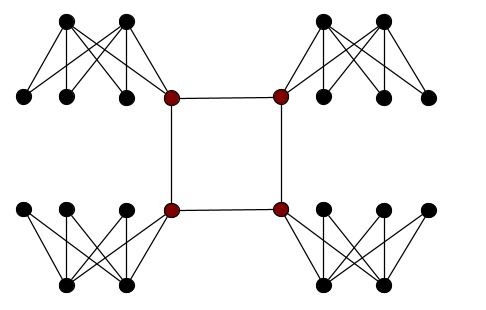
\includegraphics[width=5.5cm]{./img/Qexemplo}    
    & &
   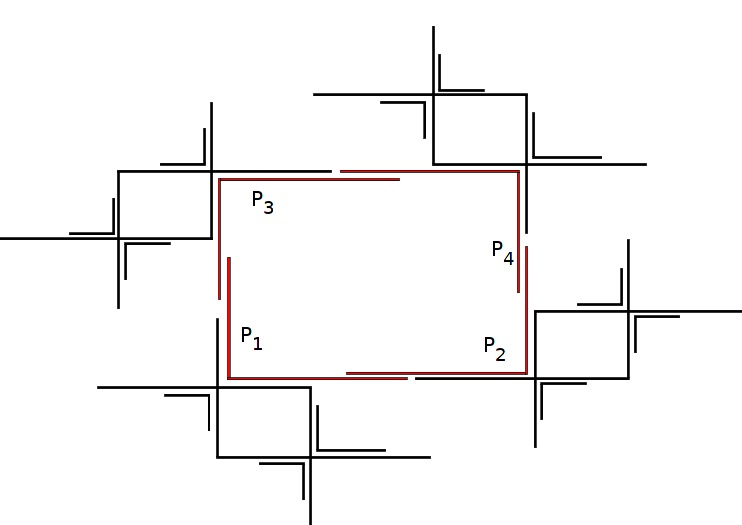
\includegraphics[width=8cm]{./img/representationQ}
  \end{tabular}
  \caption{A bat graph $G$ and a Helly-$B_1$-EPG representation of $G$.}\label{fig:grafoQ}
\end{figure} 

\begin{corollary}\label{batgraph}
In every single bend representation of the bat graph, $G$ presented in Fig.~\ref{fig:grafoQ}, the $C_4$ that is a transversal of all $K_{2,4}$ is represented by a square-frame.
\end{corollary}


\begin{figure}[htb]
  \centering
  \begin{tabular}{c c c c c }
   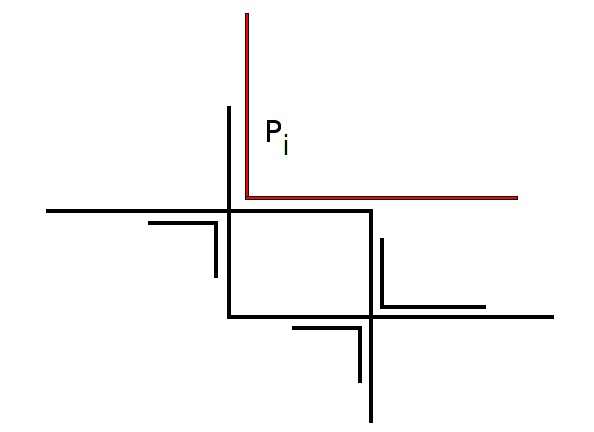
\includegraphics[width=5cm]{./img/representationQ2}
  \end{tabular}
  \caption{Helly-$B_1$-EPG representation of a $K_{2,4}$.}\label{fig:grafoQ2}
\end{figure} 

Figure~\ref{fig:grafoQ2} is an $B_1$-EPG representation for a $K_{2,4}$ graph. We know that any representation of a $K_{2,4}$ has the same shape for vertices in largest set, i.e. bending in a false pie. This fact is fundamental for the construction of a $B_1$-EPG representation of the bat graph, see Figure~\ref{batgraph}. When  we positioned a path $P_i$ corresponding to a vertex of the largest part of $K_{2,4}$ in construction of the bat graph, then we can state that the bend edge of each path $P_i$ does not be used by any non-member of this $K_{2,4}$. Thus each $P_i$ has to intersect another members of this $C_4$ by an extremity edge. Thus, we conclude that each path representing a vertex of the $C_4$ (transversal to all $K_{2,4}$) has its bend in a false pie and this $C_4$ is represented by a square-frame.

\begin{definition}
A $B_k$-EPG representation is \emph{minimal} 
when its set of edges does not properly contain another $B_k$-EPG representation. 
\end{definition}

The \textit{octahedral} graph is the graph containing 6 vertices and 12 edges, depicted  in Figure~\ref{fig:octaedro}(a). Next, we consider representations of the octahedral graph.
 

The next lemma follows directly from the discussion presented in~\cite{heldt2014}.

\begin{lemma}\label{lem:octaedronaohelly}
Every minimal $B_1$-EPG representation of the octahedral graph $O_3$ has the same shape.
\end{lemma}

 
\begin{figure}[h]
  \centering
  
%segundo bloco de figuras
  \begin{tabular}{@{}c@{} p{1.5cm} @{}c@{} }
   \centering 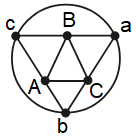
\includegraphics[width=2.5cm]{./img/octaedro.png} & &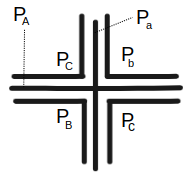
\includegraphics[width=4cm]{./img/representacaoOctaedro.png}  \\[\abovecaptionskip]
    \footnotesize \centering (a) O grafo octaedro $O_3$   & &  \footnotesize(b) Representação $B_1$-EPG do grafo $O_3$
  \end{tabular}

 \caption{O grafo octaedro $O_3$ e sua representação $B_1$-EPG}\label{fig:octaedro}
\end{figure}

The true pie presented in Figure~\ref{fig:octaedro}(b) is composite by paths corresponding to the vertex set $\{b, B, c, C\}$ of the Figure~\ref{fig:octaedro}(a). But in another $B_1$-EPG representation other paths corresponding to a different set of vertices could form the true pie, in any case, yet the shape is maintained. 



\section{Subclasses of $B_1$-EPG graphs}


By Lemma~\ref{lem:octaedronaohelly}, every minimal $B_1$-EPG representation of the octahedral graph $O_3$ has the same shape, as depicted in Fig.~\ref{fig:octaedro}(b). 
Since in any representation of the graph $O_3$ there is always a triple of paths that do not satisfy the Helly property, paths $P_{a}, P_{b} $ and $P_{c}$ in the case of Fig.~\ref{fig:octaedro}(b), it holds that $O_3 \notin$ Helly-$B_1$ EPG, which implies that the class of Helly-$B_1$-EPG graphs is a proper subclass of $B_1$-EPG.

It is easy to see that any $B_0$-EPG representation is Helly. Thus, $B_0$-EPG and Helly-$B_0$-EPG graphs coincide.  Hence, Helly-$B_0$ EPG can be recognized in polynomial time, see \cite{booth1976}.

In a $B_1$-EPG representation of a graph, the paths can be of the following four shapes: $\llcorner$, $\lrcorner$, $\ulcorner$ and $\urcorner$. \citet{cameron2016edge} studied $B_1$-EPG graphs whose paths on the grid belong to a proper subset of the four shapes. If $S$ is a subset of $\{\llcorner, \lrcorner, \ulcorner, \urcorner\}$, then $[S]$ denotes the class of graphs that can be represented by paths whose shapes belong to $S$, where zero-bend paths are considered to be degenerate $\llcorner$'s. They consider the natural subclasses of $B_1$-EPG: $[\llcorner], [\llcorner, \ulcorner], [\llcorner, \urcorner]$ and $[\llcorner, \ulcorner, \urcorner]$, all other subsets are isomorphic
to these up to 90 degree rotation. \cite{cameron2016edge}  showed that recognizing each of these classes is NP-complete.

The following shows how these classes relate to the class of Helly-$B_1$-EPG graphs.
%%%%%%%%%%%%%%

%\begin{figure}[htb]	
\center%6.3
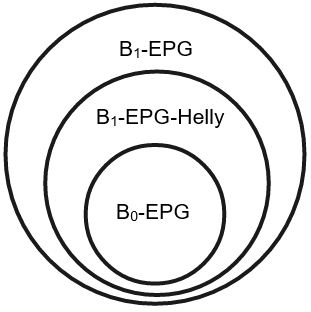
\includegraphics[width=3.5cm]{./img/diagramaClassesEPG.png}
\caption{Diagrama hierárquico de algumas classes  EPG}
\label{fig:diagramaEPG}
\end{figure}
\begin{figure}[H]	
\center%6.3
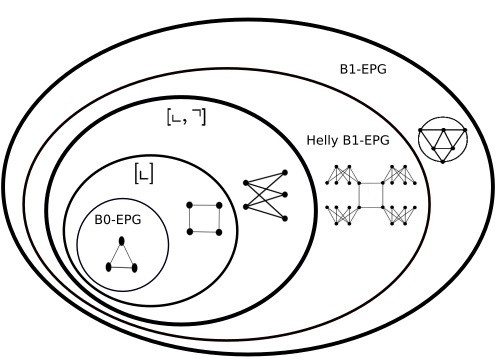
\includegraphics[width=8.5cm]{./img/classes} %2
\caption{Hierarchical diagram of some EPG classes.}
\label{fig:diagramaEPG}
\end{figure}

\begin{theorem}\label{theo:HellyLShaped}
$[\llcorner]\subsetneq [\llcorner, \urcorner]\subsetneq$~Helly-$B_1$ EPG, and Helly-$B_1$ EPG is incomparable with $[\llcorner, \ulcorner]$ and $[\llcorner, \ulcorner, \urcorner]$.
\end{theorem}

The demonstration of Theorem~\ref{theo:HellyLShaped} use statements of \cite{cameron2016edge} about $L$-shaped paths, it also use the bat graph representation (see Fig.~\ref{fig:grafoQ}) and Corollary~\ref{batgraph} and results known to Helly graphs. 

Figure~\ref{fig:diagramaEPG} depicts example of graphs of the classes $B_0$-EPG, $[\llcorner]$, $[\llcorner, \urcorner]$, Helly-$B_1$ EPG, and $B_1$-EPG that distinguish these classes.

It is known that recognizing $[\llcorner]$, $[\llcorner, \urcorner]$, and $B_1$-EPG are NP-complete while recognizing $B_0$-EPG and EPG graphs can be done in polynomial time (c.f.~\cite{booth1976}, \cite{heldt2014}, and \cite{cameron2016edge}).

Although the classes $ B_1$-EPG and Helly-$B_1$ EPG are distinct, the same is not true for the classes $B_0$-EPG and Helly-$B_0 $ EPG, because any $B_0$-EPG representation is Helly.  The $B_0$-EPG class corresponds exactly to class of interval graphs, see~\citet{booth1976}. Throughout the text we will show that each class of Helly-$B_k$ EPG is contained in the corresponding non-Helly class for all $ k \geq 1$, i.e. Helly-$B_k$ EPG $ \subsetneq$ $B_k$-EPG.

In following sections we show that it is NP-complete to recognize Helly-$B_1$-EPG graphs.


\section{Membership in $\mathcal{NP}$} \label{sec:NPpert}

%In this paper we are interested in characterizing the complexity of the $B_1$-EPG-Helly recognition problem, whose formal definition is presented next:
In this section, we will show that the (Helly-)$B_k$-EPG graph recognition problem belongs to $\mathcal{NP}$, when $k$ is polynomial in size with respect to $ |V(G)|$. The problem can be formally described as follows.

% \begin{table}[h!]
% \centering
% %\caption{My caption}
% %\label{my-label}
% \begin{tabular}{ll}
% \hline \hline
% \multicolumn{2}{c}{\sc Reconhecimento $B_k$-EPG-Helly}                         \\ \hline \hline 
% \emph{Entrada}: & Um grafo $G$, e um inteiro $k$.\\
%  & \\
% \emph{Objetivo}: & \begin{tabular}[c]{@{}p{12.5cm}}
% Determinar se existe um conjunto de caminhos $\mathcal{P} = \{P_1, P_2, \ldots, P_n\}$, com até $k$-dobras,  em uma grade  $ Q $ 
% tal que: \\
% \ \ $\bullet$ $v_i, v_j\in V(G)$ são adjacentes se e somente se  $P_i,P_j$ compartilham uma aresta em $Q$; \\
% \ \ $\bullet$ $\mathcal{P}$ satisfaz à propriedade Helly.
% \end{tabular} \\ \hline
% \end{tabular}
% \end{table}



\begin{table}[h!]
\centering
%\caption{My caption}
%\label{my-label}
\begin{tabular}{ll}
\hline \hline
\multicolumn{2}{c}{\sc Helly-$B_k$ EPG Recognition}                         \\ \hline \hline 
\emph{Input}: & A graph $G$ and an integer $k \leq |V(G)|^c$, for some fixed $c$.\\
~ & ~ \\
\emph{Goal:}  & \begin{tabular}[c]{@{}p{9.5cm}}
Determine if there is a set of $k$-bend paths \\ $\mathcal{P} = \{P_1, P_2, \ldots, P_n\} $ in a grid $ Q $ 
such that:\\ 
$\bullet$ \ \ \ $u,v\in V(G)$ are adjacent in $G$ if only if $P_u,P_v$\\ \hspace{0.6cm} share an edge in $Q$; and\\
$\bullet$ \ \ \ $\mathcal{P}$ satisfies the Helly property.
\end{tabular} \\ \hline
\end{tabular}
\end{table}


A (positive) certificate for the {\sc Helly-$B_k$ EPG recognition} consists of a grid $Q$, a set $\mathcal{P}$ of $k$-bend paths on $Q$, which is in one-to-one correspondence with the vertex set $V(G)$ of $G$, such that, for each pair of distinct paths $P_i, P_j\in \mathcal{P}, P_i\cap P_j \neq \emptyset $ if and only if the corresponding vertices are adjacent in $G$. Furthermore, $\mathcal{P}$ satisfies the Helly property.


The following are key concepts that make it easier to control the size of an EPG representation. A \emph{relevant edge} of a path in a $B_k$-EPG representation is either an extremity edge or a bend edge of the path. Note that each path with at most $k$ bends can have up to $2(k + 1)$ relevant edges, and any $B_k$-EPG representation contains at most $2|\mathcal{P}|(k + 1)$ distinct relevant edges. 


To show that there is a non-deterministic polynomial-time algorithm for {\sc Helly-$B_k$ EPG recognition}, it is enough to consider as certificate a  $B_k$-EPG representation $R$ containing a collection $\mathcal{P}$ of paths, $|\mathcal{P}| = |V(G)|$, such that  each path $P_i \in \mathcal{P}$ is given by its set of relevant edges along with the relevant edges, that intersects $P_i$, of each path $P_j$ intersecting $P_i$, where $P_j \in \mathcal{P}$.  The relevant edges for each path are given in the order that they appear in the path, to make straightforward checking that the edges correspond to a unique path with at most $k$ bends.  This representation is also handy for checking that the paths form an intersection model for $G$.

To verify in polynomial time that the input is a positive certificate for the problem, we must assert the following:

\begin{enumerate}%[label=(\roman*)]
\item[(i)] The sequence of relevant edges of a path $P_i\in \mathcal{P}$ determines $P_i$ in polynomial time; \label{it:bullet1}

\item[(ii)] Two paths $P_i, P_j \in \mathcal{P}$ intersect if and only if they intersect in some relevant edge; \label{it:bullet2}

\item[(iii)] The set $\mathcal{P}$ of relevant edges satisfies the Helly property.  \label{it:bullet3}
\end{enumerate}


%The following lemma shows condition~\ref{it:bullet1} holds.

The following lemma states that condition~(i) holds. 



\begin{lemma}\label{lem:verify1}
Each path $P_i$ can be uniquely determined in polynomial time by the sequence of its relevant edges.
\end{lemma}
% \begin{proof}
% Consider the sequence of relevant edges of some path $P_i\in \mathcal{P}$. Start from an extremity edge of $P_i$. Let $t$ be the row (column) containing the last considered relevant edge. The next relevant edge $e'$ in the sequence, must be also contained in row (column) $t$. If $e'$ is an extremity edge, the process is finished, and the path has been determined. It contains all edges between the considered relevant edges in the sequence. Otherwise, if $e'$ is a bend edge, the next relevant edge is the second bend edge $e''$ of this same bend, which is contained in some column (row) $t'$. The process continues until the second extremity edge of $P_i$ is located. 

% With the above procedure, we can determine in $\mathcal{O}(k\cdot |V(G)|)$ time, whether path $P_i$ contains any given edge of the grid $Q$. Therefore, the sequence of relevant edges of $P_i$ uniquely determines $P_i$.
%  \end{proof}

Next, we assert property~(ii).

\begin{lemma}\label{lem:relevantEdges}
Let $\mathcal{P}$ be the set of paths in a $B_k$-EPG representation of $G$, and let $P_1, P_2\in \mathcal{P}$. Then $P_1$, $P_2$ are intersecting paths if and only if their intersection contains at least one relevant edge.
\end{lemma}

% \begin{proof}
%  Assume that $P_1, P_2$ are intersecting, and we show they contain a common relevant edge. Without loss of generality, suppose $P_1, P_2$ intersect at row \textit{i} of the grid, in the  $B_k$-EPG representation $R$. The following are the possible cases that may occur:

% \begin{itemize}
% \item \textbf{Case 1:} Neither $P_1$ nor $P_2$ contain bends in row \textit{i}. 

% Then $P_1$ and $ P_2$  are entirely contained in row \textit{i}. Since they intersect, either $P_1, P_2$  overlap, or one of the paths contains the other. In any of these situations, they intersect in a common extremity edge, which is a relevant edge.

% \item \textbf{Case 2:} $P_1$ does not contain bends in \textit{i}, but $ P_2$ does.

% If some bend edge of $P_2$ also belongs to $P_1$, then $P_1, P_2$  intersect in  a relevant edge. Otherwise, since $P_1, P_2$  intersect, the only possibility is that the intersection contains an extremity edge of $P_1$ or $ P_2$. Hence the paths intersect in a relevant edge.  

% \item \textbf{Case 3:} Both $P_1$,  $P_2$ contain bends in \textit{i}

% Again, if the intersection occurs in some bend edge of $P_1$  or $P_2$, the lemma follows. Otherwise, the same situation as above must occur: $P_1, P_2$  must intersect in an extremity edge.
 
% \end{itemize}
% In any of the cases, $P_1$ and $P_2$ intersect in some relevant edge.
%  \end{proof}
 
 
The two previous lemmas let us check that a certificate is an actual $B_k$-EPG representation of a given graph $G$.  The next lemma says we can also verify in polynomial time that the representation encoded in the certificate is a Helly representation. Fortunately, we do not need to check every subset of intersecting paths of the representation to make sure they have a common intersection. 


\begin{lemma}\label{lem:verify3}
Let $\mathcal{P}$ be a collection of paths encoded as a sequence of relevant edges that constitute a  $B_k$-EPG representation of a graph $G$. We can verify in polynomial time if $\mathcal{P}$ has the Helly property.
\end{lemma}


% \begin{proof}
% Let $T$ be the set of relevant edges of $\mathcal{P}$. Consider each triple $T_i$ of edges of $T$ . Let $P_i$ be the set of paths of $\mathcal{P}$ containing at least two of the edges in the triple  $T_i$. By Gilmore's Theorem, see \cite{bergeDuchet1975}, $\mathcal{P}$ has the Helly property if an only if the subset of paths $P_i$  corresponding to each triple  $T_i$  has a non-empty intersection.  By Lemma~\ref{lem:relevantEdges}, it suffices to examine the intersections on relevant edges. Therefore a polynomial algorithm for checking if $\mathcal{P}$ has the Helly property could examine each of the subsets $P_i$, and for each relevant edge $e$ of a path in $P_i$, to compute the number of paths in $P_i$ that contain $e$. Then  $\mathcal{P}$ has the Helly property if and only if for every  $P_i$,  there exists some relevant edge that is present in all paths in $P_i$,  yielding a non-empty intersection.
%  \end{proof}

\begin{corollary}\label{cor:comumAtodos}
Let ${\mathcal P'}$ be a set a pairwise intersecting paths in a Helly-$B_k$-EPG representation of a graph $G$. Then the intersection of all paths of  ${\mathcal P'}$ contains at least one relevant edge.
\end{corollary}

Note that the property described in Corollary~\ref{cor:comumAtodos} is a consequence of Gilmore's Theorem, see~\cite{bergeDuchet1975}, and it applies only to representations that satisfy Helly's property.

From Corollary~\ref{cor:comumAtodos}, the following theorem concerning the Helly-bend number of a graph holds.

\begin{theorem}\label{teo:lowerboundCliques}
For every graph $G$ containing $n$ vertices and $\mu$ maximal cliques, it holds that $$\frac{\mu}{2n}-1\leq b_H(G)\leq \mu -1.$$ 
\end{theorem}
% \begin{proof}
% The upper bound follows from Corollary~\ref{cor:maxCliques}.
% For the lower bound first notice that each path with at most $k$ bends can have up to $2(k + 1)$ relevant edges, and any $B_k$-EPG representation with a set of paths $\mathcal{P}$ contains at most $2|\mathcal{P}|(k + 1)$ distinct relevant edges. Now, let $G$ be a graph with $n$ vertices, $\mu$ maximal cliques, and $b_H(G)=k$. From Corollary~\ref{cor:comumAtodos}, it follows that in a Helly-$B_k$-EPG representation of $G$ every maximal clique of $G$ contains at least one relevant edge. By maximality, two distinct maximal cliques cannot share the same edge-clique. Thus, in a Helly-$B_k$-EPG representation of $G$ every maximal clique of $G$ contains at least one distinct relevant edge, which implies that $\mu\leq 2n(k+1)$, so $\frac{\mu}{2n}-1\leq b_H(G)$.
% \end{proof}


\begin{lemma}\label{lem:gridPolinomial}
Let $G$ be a (Helly-)$B_k$-EPG graph. Then $G$ admits a (Helly-)$B_k$-EPG representation on a grid of size at most $4n(k+1) \times 4n(k+1)$.
\end{lemma}
% \begin{proof}
% Let $R$ be a $B_k$-EPG representation of a graph $G$ on a grid $Q$ with the smallest possible size.
% Let $\mathcal{P}$ be the set of paths of $R$. Note that $|\mathcal{P}|=n$.
% A counting argument shows that there are at most $2|\mathcal{P}|(k+1)$ relevant edges in $R$. 
%  If $Q$ has a pair of consecutive columns $c_i,c_{i+1}$ neither of which contains relevant edges of $R$, and such that there is no relevant edge crossing from $c_i$ to $c_{i+1}$, then we can contract each edge crossing from $c_i$ to $c_{i+1}$ into single vertices so as to obtain a new  $B_k$-EPG representation of $G$ on a smaller grid, which is a contradiction. An analogous argument can be applied to pairs of consecutive rows of the grid.
%  Therefore the grid $Q$ is such that each pair of consecutive columns and consecutive rows of $Q$  has at least one relevant edge of $R$ or contains a relevant edge crossing it.  
%   Since $Q$ is the smallest possible grid for representing $G$, then the first row and the first column of $Q$ must contain at least one point belonging to some relevant edge of $R$. 
% Thus, if $G$ is $B_k$-EPG then it admits a $B_k$-EPG representation on a grid of size at most $4|\mathcal{P}|(k+1) \times 4|\mathcal{P}|(k+1)$.
% Besides, by Corollary~\ref{cor:comumAtodos}, it holds that the contraction operation previously described preserves the Helly property, if any. Hence, letting $R$ be a Helly-$B_k$-EPG representation of a graph $G$ on a grid $Q$ with the smallest possible size it holds that $Q$ has size at most $4|\mathcal{P}|(k+1) \times 4|\mathcal{P}|(k+1)$.\end{proof}

Given a graph $G$ with $n$ vertices and an EPG representation $R$, it is easy to check in polynomial time with respect to $n +|R|$ whether $R$ is a $B_k$-EPG representation of $G$. By Lemma~\ref{lem:gridPolinomial}, if $G$ is a $B_k$-EPG graph then there is a positive certificate (an EPG representation) $R$ of polynomial size  with respect to $k+n$ to the question ``$G\in B_k$-EPG?''. Therefore, Corollary~\ref{BkNP} holds.

\begin{corollary}\label{BkNP}
Given a graph $G$ and an integer $k\geq 0$, the problem of determining whether $G$ is a $B_k$-EPG graph is in NP, whenever $k$ is bounded by a polynomial function of $|V(G)|$.
\end{corollary}

At this point, we are ready to demonstrate the NP-membership of {\sc Helly-$B_k$ EPG recognition}.

\medskip

\begin{theorem}\label{teo:nppertinencia}
{\sc Helly-$B_k$ EPG recognition} is in NP.
\end{theorem}
% \begin{proof}
% By Lemma~\ref{lem:gridPolinomial} and the fact that $k$ is bounded by a polynomial function of $|V(G)|$, it follows that the collection $\mathcal{P}$ can be encoded through its relevant edges with $n^{\mathcal{O}(1)}$ bits.

% Finally, by Lemmas~\ref{lem:verify1}, \ref{lem:relevantEdges} and \ref{lem:verify3}, it follows that one can verify in polynomial-time in the size of $G$ whether $\mathcal{P}$ is a family of paths encoded as a sequence of relevant edges that constitute a Helly-$B_k$-EPG representation of a graph $G$.
% \end{proof}

\section{$NP$-Hardness}\label{sec:sectionDispositivoClausula}

Now we will prove that  {\sc Helly-$B_1$ EPG recognition} is NP-complete. For this proof, we follow the basic strategy described in the prior hardness proof of~\cite{heldt2014}. We set up a reduction from {\sc Positive (1 in 3)-3SAT} defined  as follows:

\begin{table}[h!]
\centering
%\caption{My caption}
%\label{my-label}
\begin{tabular}{ll}
\hline \hline
\multicolumn{2}{c}{\sc Positive (1 in 3)-3SAT}                                \\ \hline \hline 
\emph{Entrada}: & \begin{tabular}[c]{@{}p{12.5cm}@{}} Um conjunto $X$ de variáveis positivas; uma coleção $\mathcal{C}=\{C_1,C_2,\ldots,C_m\}$ de cláusulas sobre  $X$ tal que para cada $C_i\in \mathcal{C}$, $|C_i|= 3$.
\end{tabular} \\
 &  \\
\emph{Objetivo}:  & \begin{tabular}[c]{@{}l@{}} %@{}l@{}
Determinar se existe uma atribuição de valores para as variáveis em $ X $\\ de modo que toda cláusula em  $\mathcal{C}$ tem exatamente um literal verdadeiro.
\end{tabular} \\ \hline
\end{tabular}
\end{table}

{\sc Positive (1 in 3)-3SAT } is a well-known NP-complete problem (see \cite{johnson1979}, problem [L04], page 259). Also, it remains NP-complete when the incidence graph of the input CNF (Conjunctive Normal Form) formula is planar, see~\cite{mulzer2008minimum}.

Given a formula $F$ that is an instance of {\sc Positive (1 in 3)-3SAT} we will present a polynomial-time construction of a graph $ G_F$ such that $ G_F \in$ Helly-$B_1$ EPG if and only if $ F $ is satisfiable. This graph will contain an induced subgraph $ G_{C_i}$ with 12 vertices (called \emph {clause gadget}) for every clause $C_i \in \mathcal{C}$, and an induced subgraph (\emph {variable gadget}) for each variable $ x_j$, containing a special vertex  $ v_j$, plus a \emph{base gadget}  with 55 additional vertices.

 
We will use a graph $H$ isomorphic to the graph presented in Figure~\ref{fig:gadgetBase}, as a gadget to perform the proof. For each clause $C_i$ of $F$ of the target problem, we will have a \emph{clause gadget} isomorphic to $H$, denoted by $G_{c_i}$.

\begin{figure}[htb]	
\center%6.3
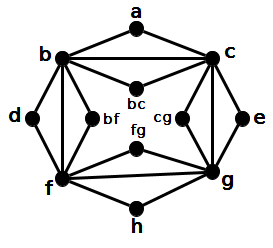
\includegraphics[width=5cm]{./img/gadgetBase.png}
\caption{The partial gadget graph $H$.}
\label{fig:gadgetBase}
\end{figure} 


The reduction of a formula $F$ from  {\sc Positive (1 in 3)-3SAT}  to a particular graph $G_F$ (where $G_F$ has a Helly-$B_1$-EPG representation if only if $F$ is satisfiable) is given below.

\begin{definition}\label{sec:reducao}
Let $F$ be a CNF-formula with variable set $\mathcal{X}$ and clause set $\mathcal{C}$ with no negative literals, in which every clause has exactly three literals. The graph $G_F$ is constructed as follows:

\begin{enumerate}
\item For each clause $C_i \in \mathcal{C}$ create a  \textit{clause gadget} $G_{C_i}$, isomorphic to  graph $H$;

\item For each variable $x_{j}\in \mathcal{X}$ create a \emph{variable vertex} $v_{j}$ that is adjacent to the vertex $a$, $e,$ or $h$ of $G_{C_i}$, when $x_{j}$ is the first, second or third variable in $C_i$, respectively;

\item For each variable vertex $v_{j}$, construct a \emph{variable gadget} formed by adding two copies of $H$, $H_1$ and $H_2$, and making $v_j$ adjacent to the vertices of the triangles $(a, b, c)$ in  $H_1$ and $H_2$.

 %where $v_{j}$ is  adjacent to all vertices of the triangle (a,b,c);%; (c,e,g); (g,f,h); or (b,d,f)) of each $H_1$ and $H_2$; 

%\item The  subgraph induced by \emph{variable vertex}  $v_{j}$, and also $V(H_1)$ and $V(H_2)$ will be called \emph{variable gadget}; 

\item Create a vertex $V$, that will be used as a vertical reference of the construction, and add an edge from $V$ to each vertex $d$ of a clause gadget;%$d \in V(G_c)$;

\item Create a bipartite graph $K_{2,4}$ with a particular vertex $T$ in the largest stable set. This vertex is nominated \emph{true vertex}. Vertex $T$ is adjacent to all $v_{j}$ and also to $V$;

\item Create two  graphs isomorphic to $H$, $G_{B1}$ and $G_{B2}$. The vertex $T$ is connected to each vertex of the triangle (a,b,c) in $G_{B1}$ and $G_{B2}$;


\item Create two graphs isomorphic  to $H$, $G_{B3}$ and $G_{B4}$. The vertex $V$ is connected to each vertex of the triangle (a,b,c) in $G_{B3}$ and $G_{B4}$;

\item The  subgraph induced by the set of vertices $\{V(K_{2,4}) \cup  \{T, V\} \cup V(G_{B1}) \cup V(G_{B2}) \cup V(G_{B3}) \cup V(G_{B4})\}$ will be referred to as the  \emph{base gadget}. 
\end{enumerate}
\end{definition}


Figure~\ref{fig:exemploGrafoGF} illustrates how this construction works on a small formula. 


\begin{figure}[htb]	
\center%6.3
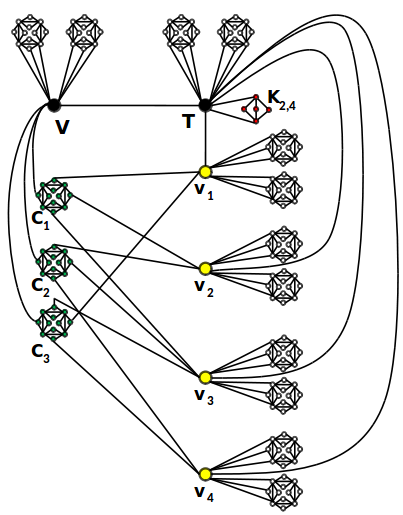
\includegraphics[width=6.5cm]{./img/exemploGrafoGFSBPO4.png}
\caption{O grafo $G_{F}$ correspondendo à fórmula $F=(x_1+ x_2+ x_3) \wedge  (x_2+ x_3+ x_4 )\wedge  (x_3 + x_1 + x_4 )$}
\label{fig:exemploGrafoGF}
\end{figure}

\begin{lemma}\label{lem:ida}
Given a satisfiable instance $F$ of {\sc Positive (1 in 3)-3SAT}, the graph $G_F$ constructed from $F$ according to Definition~\ref{sec:reducao} admits a Helly-$B_1$-EPG representation.
\end{lemma}


Using base, variables and clause gadgets constructed in an appropriate way, it is possible to demonstrate that we can obtain a Helly-$B_1$-EPG representation from the input formula. Figure~\ref{fig:gadgetFormulaCompletaPies} depicts a Helly-$B_1$-EPG representation for the gadget built in Figure~\ref{fig:exemploGrafoGF}. For more proof details see the paper is last section of this chapter.


\begin{figure}[htb]	
\center%6.3
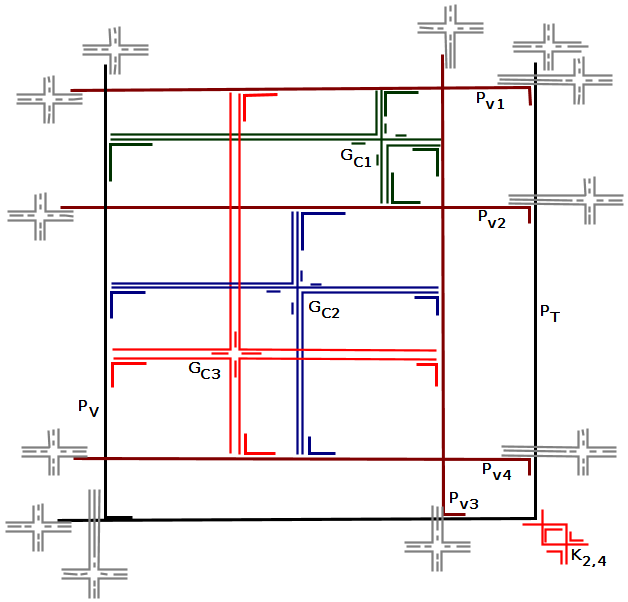
\includegraphics[width=10cm]{./img/formulaFGCompletaPies.png}
%clausulaGadgetGFCompletaSBPO
\caption{Representação de dobra simples de $G_F$}
\label{fig:gadgetFormulaCompletaPies}
\end{figure}

Now, we consider the converse. Let $R$ be a Helly-$B_1$-EPG representation of $G_F$, then we will get the original formula.


\begin{lemma}\label{lem:volta}
If a graph $G_F$, constructed according to Definition~\ref{sec:reducao}, admits a Helly-$B_1$-EPG representation, then the associated CNF-formula $F$ is a yes-instance of {\sc Positive (1 in 3)-3sat}.
\end{lemma}

To obtain the formula $F$ associated with the  representation $R$ of $G_F$, a few steps are necessary: 1 - identify the  clauses gadgets, so you can know how many clauses make up the formula; 2 - identify the variable gadgets, that way you can know which are the variables that make up each clause; 3 - check which variables and clauses gadgets have intersecting paths, so it is possible to identify which variables are in each clause; 4 - check the direction of the intersections among each variable gadget with the base gadget, this makes it possible to identify the value (True/False) of each variable.  This takes us to the next theorem.

\begin{theorem}
{\sc Helly-$B_1$ EPG recognition} is NP-complete.
\end{theorem}
\begin{proof} %\textbf{Proof}.
By Theorem~\ref{teo:nppertinencia}, Lemma~\ref{lem:ida}, Lemma~\ref{lem:volta}.
 \end{proof}



We say that a $k$-apex graph is a graph that can be made planar by the removal of $k$ vertices. A $d$-degenerate graph is a graph in which every subgraph has a vertex of degree at most $d$. Recall that {\sc Positive (1 in 3)-3SAT} remains NP-complete when the incidence graph of the input formula is planar, see~\cite{mulzer2008minimum}. Thus, the following corollary holds.

\begin{corollary}\label{coro:2apexAnd3degenerate}
{\sc Helly-$B_1$ EPG recognition} is NP-complete on $2$-apex and $3$-degenerate graphs.
\end{corollary}

To prove that $G_F$ is 3-degenerate, we apply the $d$-degenerate graphs recognition algorithm. Now, to prove that $G_F$ is $2$-appex when the incidence graph of the input formula is planar, we need to recall that {\sc Positive (1 in 3)-3SAT} remains NP-complete when the incidence graph of $F$ is planar, see~\cite{mulzer2008minimum}. Therefore, is enough to demonstrate that there is a planar arrangement between the intersections of the variable gadgets and clause gadgets, then from that one can construct a graph $G_F$ such that the removal of $V$ and $T$ results into a planar graph. The complete proof is in paper in the last section of this chapter.


\section{Concluding Remarks}

In this chapter, we show that every graph admits a Helly-EPG representation, and $\frac{\mu}{2n}-1\leq b_H(G)\leq \mu -1$. Besides, we relate Helly-$B_1$-EPG graphs with L-shaped graphs, a natural family of subclasses of $B_1$-EPG. Also, we prove that recognizing (Helly-)$B_k$-EPG graphs is in $\mathcal{NP}$, for every fixed $k$. Finally, we show that recognizing Helly-$B_1$-EPG graphs is NP-complete, and it remains NP-complete even when restricted to 2-apex and 3-degenerate graphs.

Now, let $r$ be a positive integer and let $K_{2r}^-$ be the cocktail-party graph, i.e., a complete graph on $2r$ vertices with a perfect matching removed. Since $K_{2r}^-$ has $2^r$ maximal cliques, by Theorem~\ref{teo:lowerboundCliques} follows that $\frac{2^r}{4r}-1\leq b_H(K_{2r}^-)$. This implies that, for each $k$, the graph $K_{2(k+5)}^-$ is not a Helly-$B_k$-EPG graph. Therefore, as \cite{martin2017} showed that every cocktail-party graph is in $B_2$-EPG, we conclude the following.

\begin{lemma}
Helly-$B_k$-EPG $\subsetneq B_k$-EPG for each $k>0$.
\end{lemma}

The previous lemma suggests asking about the complexity of recognizing Helly-$B_k$-EPG graphs for each $k>1$. Also, it seems interesting to present characterizations for Helly-$B_k$-EPG representations similar to Lemma~\ref{caracterization} (especially for $k=2$) as well as considering the $h$-Helly-$B_k$ EPG graphs. Regarding L-shaped graphs, it also seems interesting to analyse the classes Helly-$[\llcorner, \ulcorner]$ and Helly-$[\llcorner, \ulcorner, \urcorner]$ (recall Thereom~\ref{theo:HellyLShaped}).




\section{Article accepted for publication in the journal  Discrete Mathematics \& Theoretical Computer Science (DMTCS)} 
%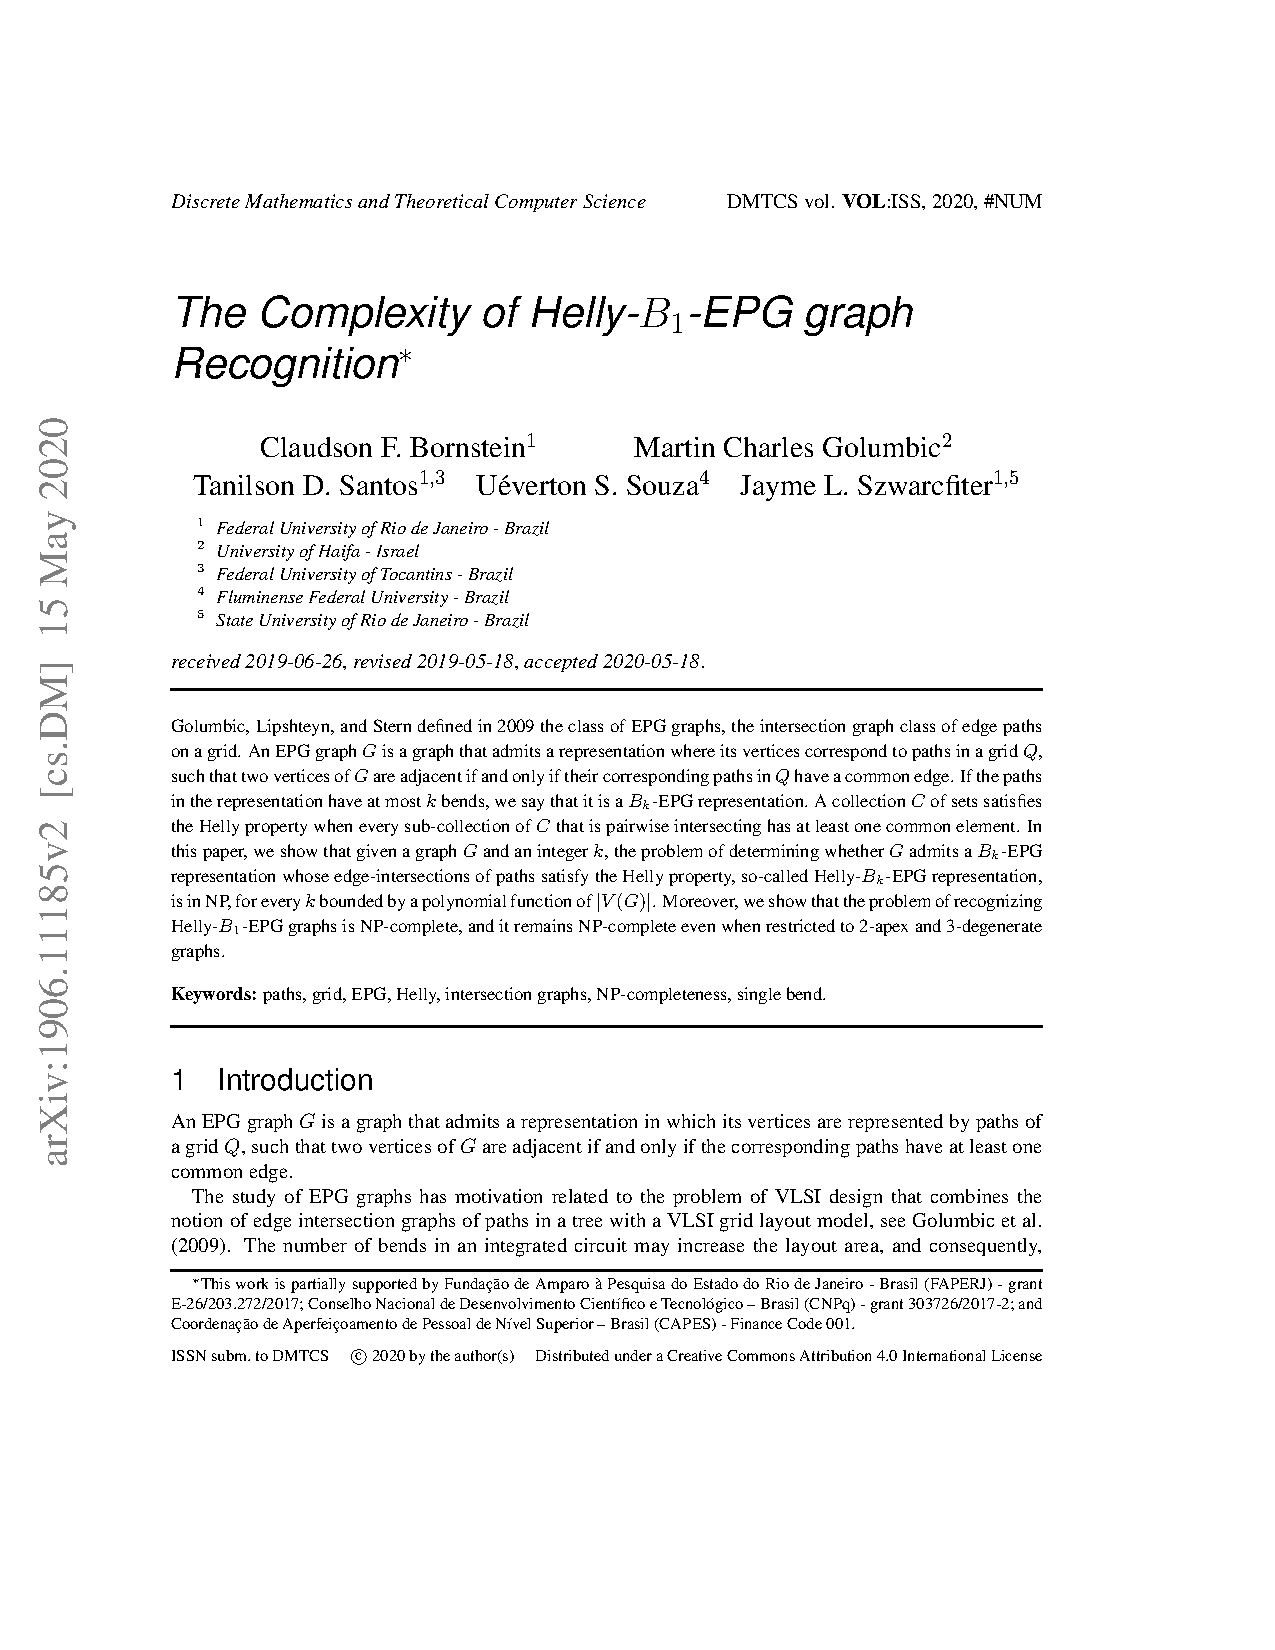
\includepdf[pages=-]{./includes/include-pdf-files/dmtcsTanilson.pdf}

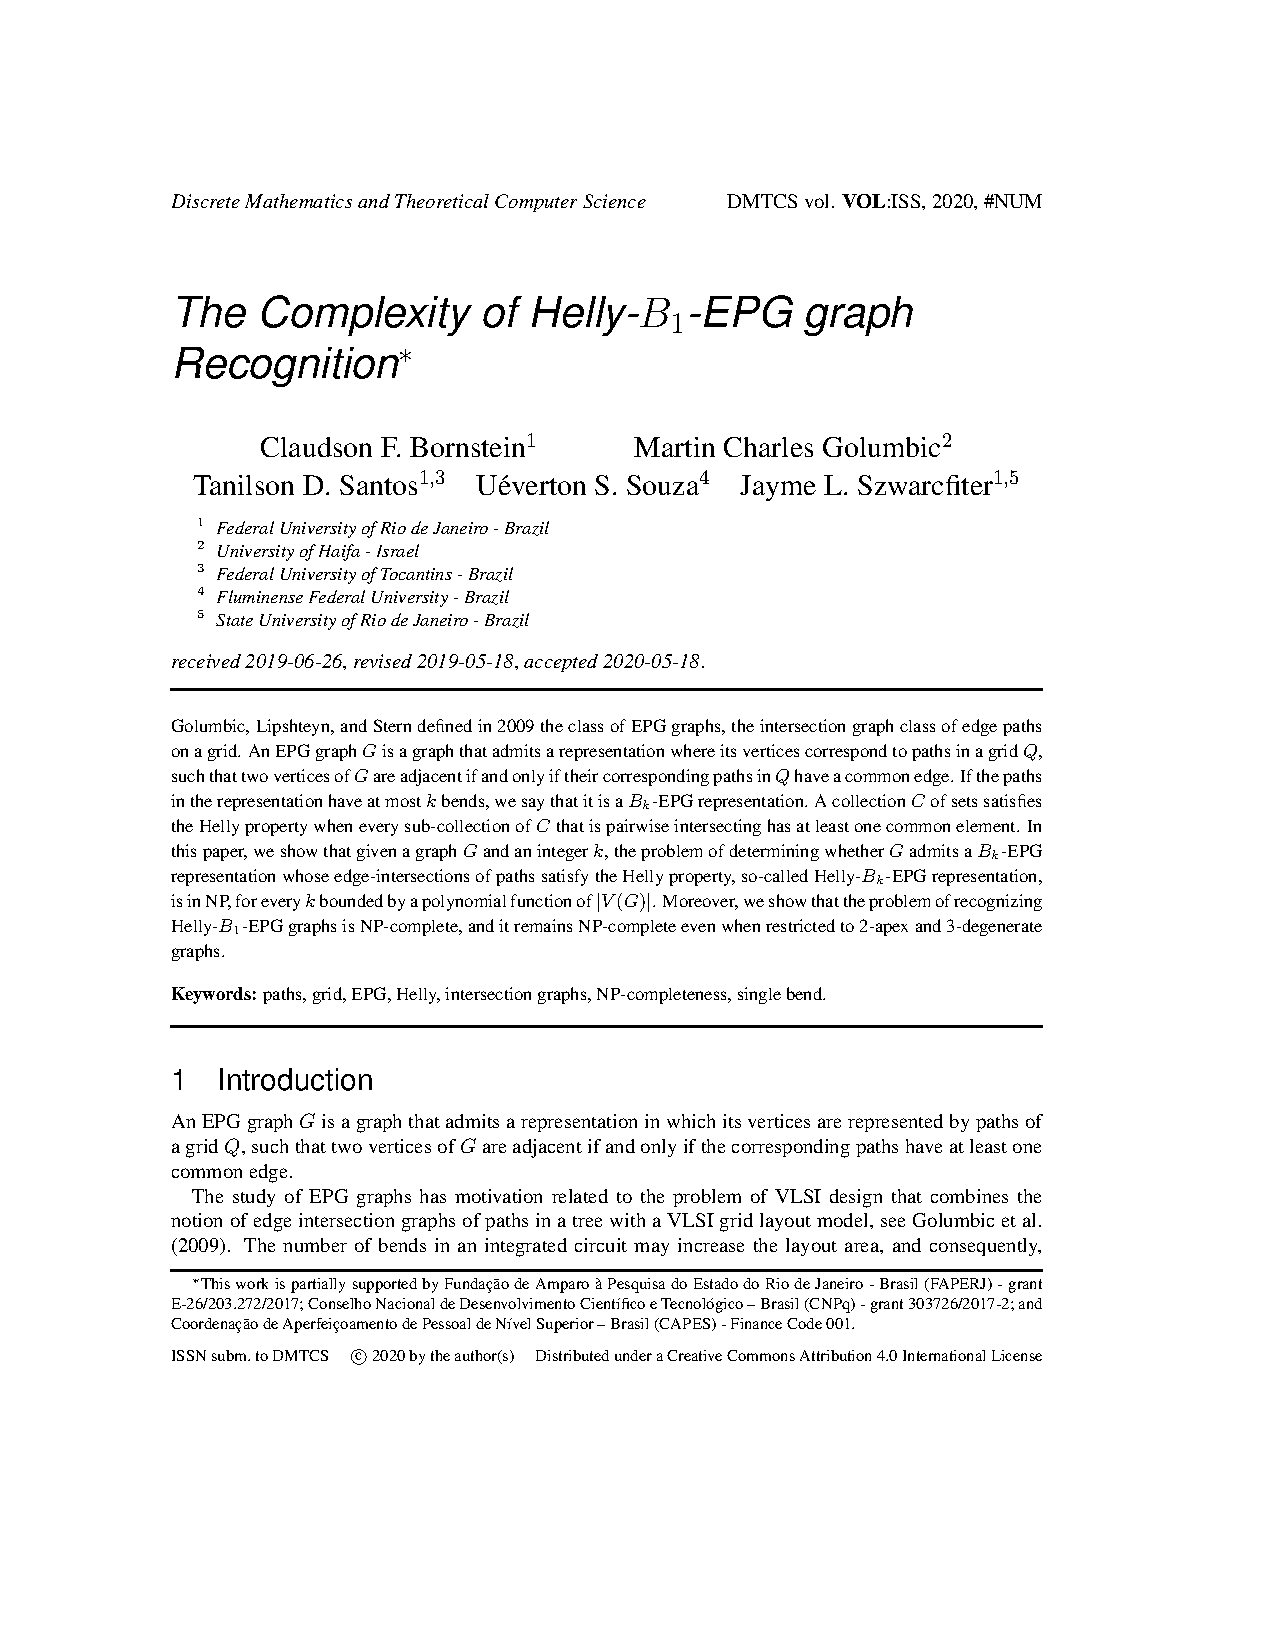
\includepdf[pages=-]{./includes/include-pdf-files/dmtcsTanilson2.pdf}